% Compile this standalone figure with pdflatex.
% Replace each \pending with the observed count after screening.
\documentclass[tikz,border=4pt]{standalone}
\usepackage[T1]{fontenc}
\usepackage{lmodern}
\usetikzlibrary{arrows.meta,positioning}
\definecolor{ink}{HTML}{173B46}
\definecolor{accent}{HTML}{147267}
\definecolor{wash}{HTML}{EFF7F5}
\newcommand{\pending}{\rule{1.5em}{0.35pt}}
\begin{document}
\sffamily
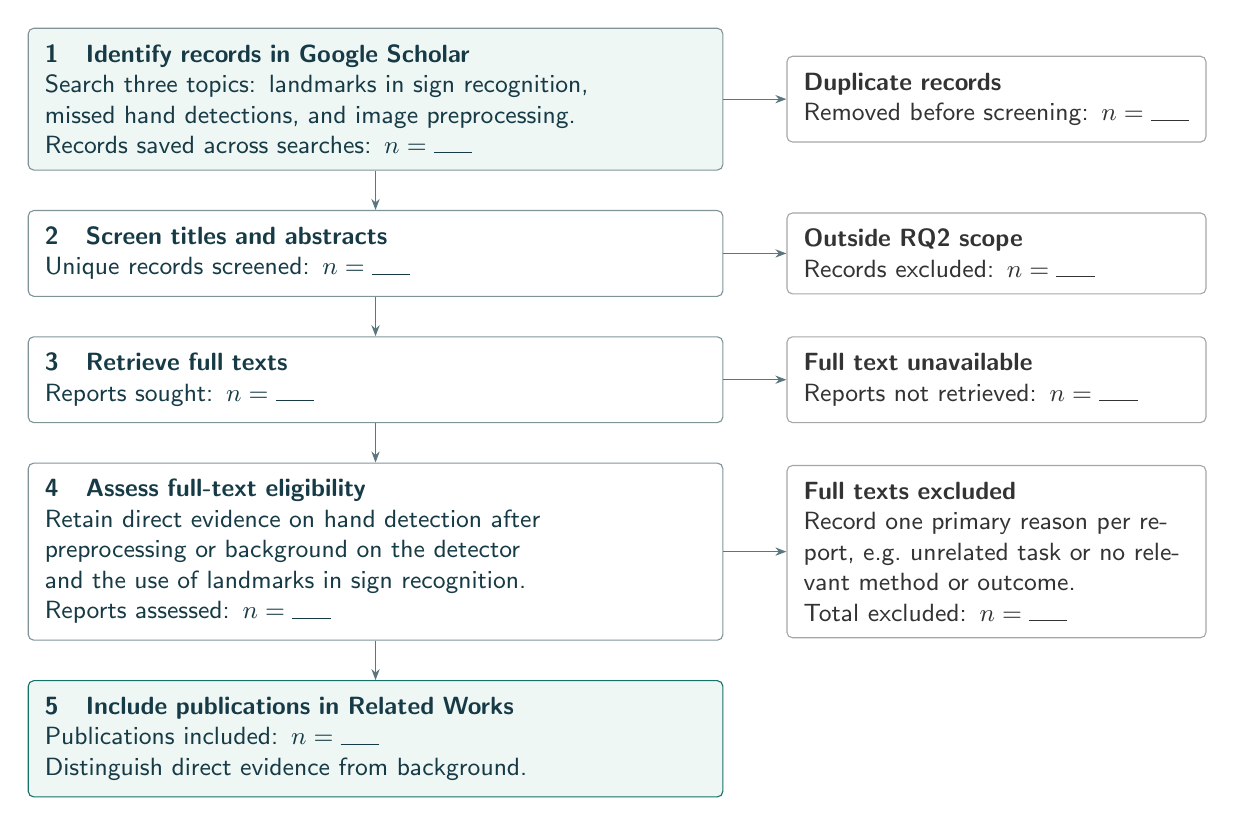
\begin{tikzpicture}[
  box/.style={draw=ink!55,rounded corners=2pt,align=left,inner sep=6pt,
              text width=84mm,text=ink,font=\small\sffamily},
  side/.style={box,text width=49mm,draw=black!35,text=black!80},
  flow/.style={-{Stealth[length=4pt]},draw=ink!70},
  node distance=5mm and 8mm]
\node[box,fill=wash] (search) {\textbf{1\quad Identify records in Google Scholar}\\
  Search three topics: landmarks in sign recognition,\\
  missed hand detections, and image preprocessing.\\
  Records saved across searches: \(n=\pending\)};
\node[side,right=of search] (dup) {\textbf{Duplicate records}\\
  Removed before screening: \(n=\pending\)};
\node[box,below=of search] (screen) {\textbf{2\quad Screen titles and abstracts}\\
  Unique records screened: \(n=\pending\)};
\node[side,right=of screen] (off) {\textbf{Outside RQ2 scope}\\
  Records excluded: \(n=\pending\)};
\node[box,below=of screen] (retrieve) {\textbf{3\quad Retrieve full texts}\\
  Reports sought: \(n=\pending\)};
\node[side,right=of retrieve] (missing) {\textbf{Full text unavailable}\\
  Reports not retrieved: \(n=\pending\)};
\node[box,below=of retrieve] (assess) {\textbf{4\quad Assess full-text eligibility}\\
  Retain direct evidence on hand detection after\\
  preprocessing or background on the detector\\
  and the use of landmarks in sign recognition.\\
  Reports assessed: \(n=\pending\)};
\node[side,right=of assess] (exclude) {\textbf{Full texts excluded}\\
  Record one primary reason per report, e.g.\ unrelated task or no relevant method or outcome.\\
  Total excluded: \(n=\pending\)};
\node[box,below=of assess,fill=wash,draw=accent] (include) {\textbf{5\quad Include publications in Related Works}\\
  Publications included: \(n=\pending\)\\
  Distinguish direct evidence from background.};
\foreach \a/\b in {search/screen,screen/retrieve,retrieve/assess,assess/include}
  \draw[flow] (\a.south) -- (\b.north);
\foreach \a/\b in {search/dup,screen/off,retrieve/missing,assess/exclude}
  \draw[flow] (\a.east) -- (\b.west);
\end{tikzpicture}
\end{document}
